\documentclass{article}

% Package Declarations
\usepackage{arxiv}
\usepackage[utf8]{inputenc} % allow utf-8 input
\usepackage[T1]{fontenc}    % use 8-bit T1 fonts
\usepackage{hyperref}       % hyperlinks
\usepackage{url}            % simple URL typesetting
\usepackage{booktabs}       % professional-quality tables
\usepackage{amsfonts}       % blackboard math symbols
\usepackage{nicefrac}       % compact symbols for 1/2, etc.
\usepackage{microtype}      % microtypography
\usepackage{lipsum}         % Lorem Ipsum fill text
\usepackage{multicol}       % Support for Multi columns for tables
\usepackage{multirow}       % Support for Multi rows fot tables
\usepackage{mathtools}      % Advanced mathtools
\usepackage{caption}        % Advanced caption configuration
\usepackage{amsmath}        % Math package for equations       
\usepackage{titlesec}       % Title section
\usepackage{graphicx}       % For adding labels to parts of the equation
\usepackage{stackrel}       % For adding labels to parts of the equation
\usepackage[ruled,vlined]{algorithm2e}  % For Algorithms
\usepackage{algorithm}
\usepackage{algpseudocode}


% Theme Configurations

% Set section depth to 4
% \setcounter{secnumdepth}{4}

% \titleformat{\paragraph}
% {\normalfont\normalsize\bfseries}{\theparagraph}{1em}{}
% \titlespacing*{\paragraph}
% {0pt}{3.25ex plus 1ex minus .2ex}{1.5ex plus .2ex}

% Add padding to text below table
\captionsetup[table]{skip=10pt}

% Configure hat tex
\let\oldhat\hat
\renewcommand{\hat}[1]{\oldhat{\mathbf{#1}}}

% Document Start

\title{Differentiable Learning by means of Neural Network Pruning}

\author{
  Prathyush S Parvatharaju\thanks{Use footnote for providing further
    information about author (webpage, alternative
    address)---\emph{not} for acknowledging funding agencies.} \\
  Department of Data Science\\
  Worcester Polytechnic University\\
  Worcester, MA 01609 \\
  \texttt{psparvatharaju@wpi.edu} \\
  %% examples of more authors
   \And
 Shreesha Narasimha Murthy \\
  Department of Data Science\\
  Worcester Polytechnic University\\
  Worcester, MA 01609 \\
  \texttt{snarasimhamurthy@wpi.edu} \\
}

\begin{document}
\maketitle

\begin{abstract}
The idea of linear flow i.e, each node in one layer is connected to a certain weight $\hat{W_{ij}}$ to every node in the following layer, for the deep neural network is limiting in the sense of the way we, humans think. The linear flow would be a constraint for a DNN as DNNs can process data and emulate relationships in higher dimensions. Deeper neural networks are difficult to train and the use of residual learning in the form of short-circuit connections eases the process of training the network. By replacing the linear flow constraint with a decision process of placing short-circuit connections between layers as a gradient-based approach would yield better results. We propose a novel idea of extending the capabilities of previously used short-circuits as differentiable functions, essentially solving “What to feed?”. To tackle the problem, “When to stop?” we propose an algorithm based on Information Transfer derived from differentiable short-circuits. 

In our experiments, we show that increased weighted representation capability results in achieving better accuracy in fewer iterations compared to the standard architecture. We also demonstrate that with 10\% of the previous parameters, the architecture achieves similar results to standard architecture. Another set of experiments shows our proposed architecture builds better representations with minimal data.
\end{abstract}


% keywords can be removed
\keywords{Differentiable Learning \and Pruning \and Neural Architecture Search}


\section{Introduction}
The ability to recognize patterns and develop strong relations among them has made Neural Network supersede state of the art machine learning techniques. The depth of representations is of central importance for many visual recognition tasks. Right from Alex Net \cite{Krizhevsky2012ImageNetCW} up until ResNet \cite{He2016DeepRL} the flow of data followed linear fashion i.e the data flows from one layer to the next layer and so on. ResNet brought in an innovation by creating \emph{"Short Circuits"} meaning there exists a skip connection where, as usual, data is fed to the next layer and in certain circumstances, it is fed to the layer after its immediate next. This paved way to train deep-networks as it increased the representational capability of the network by overcoming issues such as vanishing / exploding gradients \cite{Bengio1994LearningLD, Glorot2010UnderstandingTD}. In our work we set out a goal to explore the \emph{"representational capability"} and its effects on the performance of the network. This led to the question - "What to feed?".

ResNet brings in short circuits between residual components and the number of skip connections is restricted. We propose \emph{"Global Short Circuit"}(GSC) to investigate the behavior of short circuits by revoking restriction and providing skip connections from one layer to every other layer. Thereby enhancing the representational capability of the network and therefore yields better accuracy in fewer iterations compared to standard architecture (See section \ref{sssec:ffn}). However, this modification results in a large network compared to the standard architecture. Due to the increase in parameters, the network is rendered not scalable. In order to tackle this issue we propose an enhanced version of GSC i.e, \emph{" Differentiable Short Circuit"}(DSC) - a novel architecture to help network scaling by pruning unwanted connections over time.

To tackle the issue of \emph{"When to stop"}?, a novel algorithm called \emph{Information Transfer} is devised. This algorithm measures the amount of flow of data from one layer to another. Keeping track of variance in Information Transfer over iterations, based on a certain threshold, a stopping criterion is proposed.

\section{Differentiable Learning}
\label{sec:headings}

Neural networks are differentiable by nature. The standard architecture (\ref{sssec:ffn}) is static and does not change over time but, the learning changes over time. There have been efforts towards an automated way of finding the best architecture for the given data - Neural Architecture search \cite{Zoph2016NeuralAS}. The recent advent of DARTS \cite{Liu2019DARTSDA} suggests that a learning based adaptive architecture performs better compared to the static architecture. Given $N$ layers, one needs to identify the optimal data paths. The right set of combinations can be identified by using brute-force by trying out n(n-1) combinations of connections. However, as the depth of the network increases, the search space increases exponentially and training each configuration becomes a tedious and time consuming process. Gradient descent \cite{ruder2016overview} - a first order iterative search space optimization algorithm finds the local minimum of a differentiable function is used to find optimal skip connections. Initially, we describe a standard Feed forward neural network and eventually propose the Global short circuit (GSC) and Differentiable Short Circuit (DSC) architectures.

\subsection{Feed Forward Neural Network}
\label{sssec:ffn}
Multilayer perceptron trained using back-propagation \cite{Rumelhart1986LearningIR}, a supervised learning algorithm is capable of approximating solutions for complex problems. Acting as a universal approximator, the architecture has a linear flow; i.e, a layer takes the output of the immediate previous layer alone as its input.A densely connected layer provides learning features from all the combinations of the features of the previous layer. With the linear increase in the number of connections (based on the nodes in the layer) the architecture becomes scalable and time efficient. $\hat{Z}$ in Equation \ref{eq:affine_transformation} is the result of an affine transformation and is capable of learning an offset ($\hat{b}$) and a rate of correlation ($\hat{W}$) that fits the given input.

\begin{equation}
\label{eq:affine_transformation}
\begin{aligned}
\hat{Z} &= Input \cdot \hat{W} + \hat{b}&\\
\end{aligned}
\end{equation}

This type of transformation can only learn linear relationships. In order to learn any non-linearity, a squashing non-linear activation $\sigma$ \cite{Han1995TheIO} is applied to the output of each node. Sigmoid activation results in a probability as it restricts the range of the output between 0 and 1.

\begin{equation}
\label{eq:sigmoid_activation}
\begin{aligned}
\sigma(z) &= \frac{1}{1+e^{-z}} \;\;\;\;\;\;  x\in\mathbb{R}, 0<\sigma(x)<1
\end{aligned}
\end{equation}

Figure \ref{fig:SimpleFFN.png} represents standard feed forward architecture and equation \ref{eq:ffn_math_representation} is the mathematical formulation of the network. Each node in one layer is connected to a certain weight $\hat{W_{ij}}$ to every node in the following layer. 

\noindent\begin{minipage}{.45\textwidth}
   \centering
   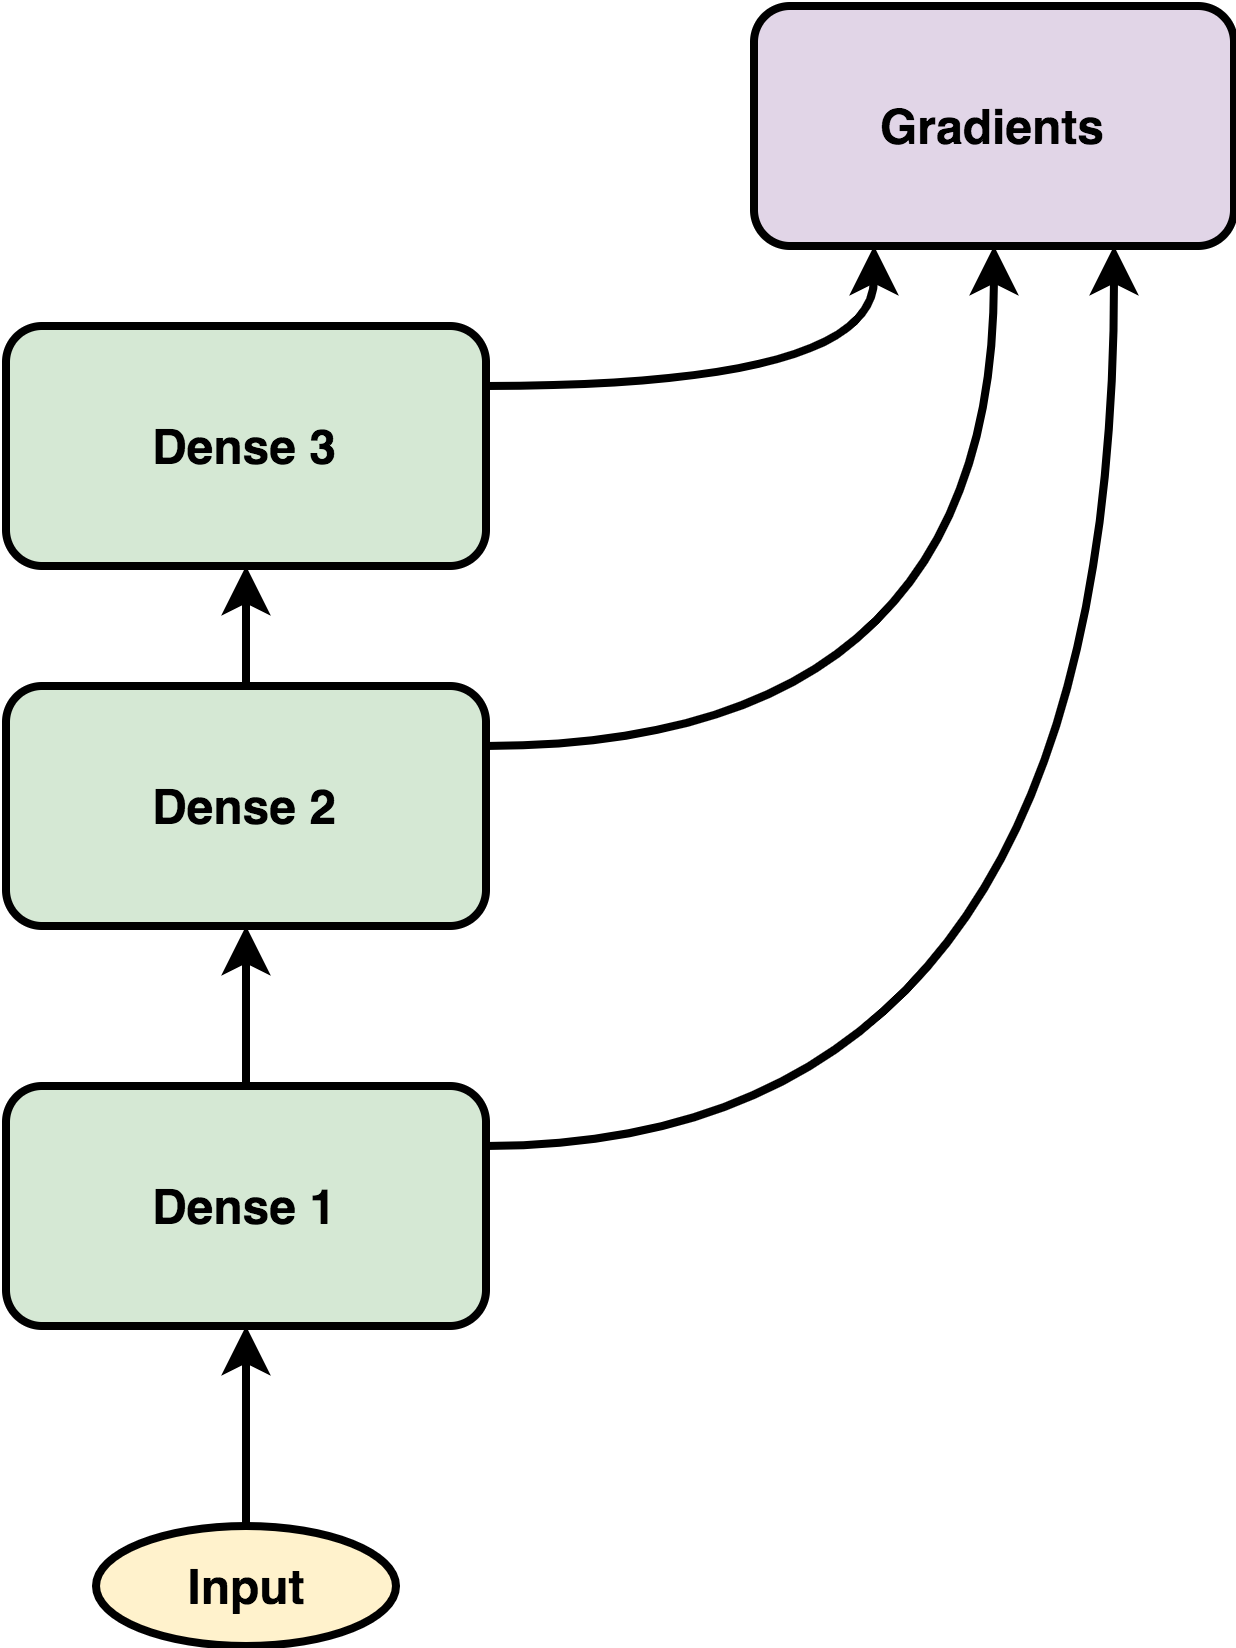
\includegraphics[scale=0.09]{SimpleFFN.png}
   \captionof{figure}{Feed Forward Network}
   \label{fig:SimpleFFN.png}
\end{minipage}
\begin{minipage}{.45\textwidth}
\begin{equation}
\label{eq:ffn_math_representation}
\begin{aligned}
   Dense_{1} &= \sigma(Input \cdot \hat{W}_{1} + \hat{b}_{1}) &\\
   Dense_{2} &= \sigma(Dense_{1} \cdot \hat{W}_{2} + \hat{b}_{2}) &\\
   Dense_{3} &= \sigma(Dense_{2} \cdot \hat{W}_{3} + \hat{b}_{3}) 
\end{aligned}
\end{equation}
\end{minipage}

For the previously mentioned standard network, the number of trainable parameters for a given layer is a function of the layer's weight, bias and input. It is represented as, 

\begin{equation}
\label{eq:ffn_params}
Params= \sum_{n=1}^{m}
\underbrace{(L_{n-1}\rule[-12pt]{0pt}{5pt}}_{\mbox{input}}
*\underbrace{L_{n})\rule[-12pt]{0pt}{5pt}}_{\mbox{weights}}
+\underbrace{L_{n}\rule[-12pt]{0pt}{5pt}}_{\mbox{bias}}
\end{equation}

For a 3 layer network with node configurations [100,50,10] and 784 input features, using equation \ref{eq:ffn_params} we arrive at 83,550 trainable parameters


\subsection{Global Short Circuit}
This work proposes the Global Short Circuit architecture to explore the impact of skip connection on representational capabilities of the network. There exists a connection from every layer to every other layer in the network. Some of the possible ways of merging layers are explored in DenseNet\cite{Li2018DenselyCC} and ResNet\cite{He2016DeepRL}. In ResNet weighted feature maps are merged using $max$ or $sum$. DenseNet merges feature using a concatenation operation. We define a merge operation similar to DenseNet's $concat$ . However, this type of merging has an issue when it comes to Convolutional Neural Networks where there is a requirement to merge feature maps of different shapes. Hence, this work proposes downsampling/padding operators to get identical shapes. Figure \ref{fig:GSC.png} shows standard architecture defined in section \ref{sssec:ffn} having connections from one layer to every other layer, merged using concat operation. The difference in the connections between the layers is relative to the number of gradient operations required for the respective layer. Equation \ref{eq:gsc_math_representation} provides mathematical representation of the architecture.

\noindent\begin{minipage}{.45\textwidth}
   \centering
   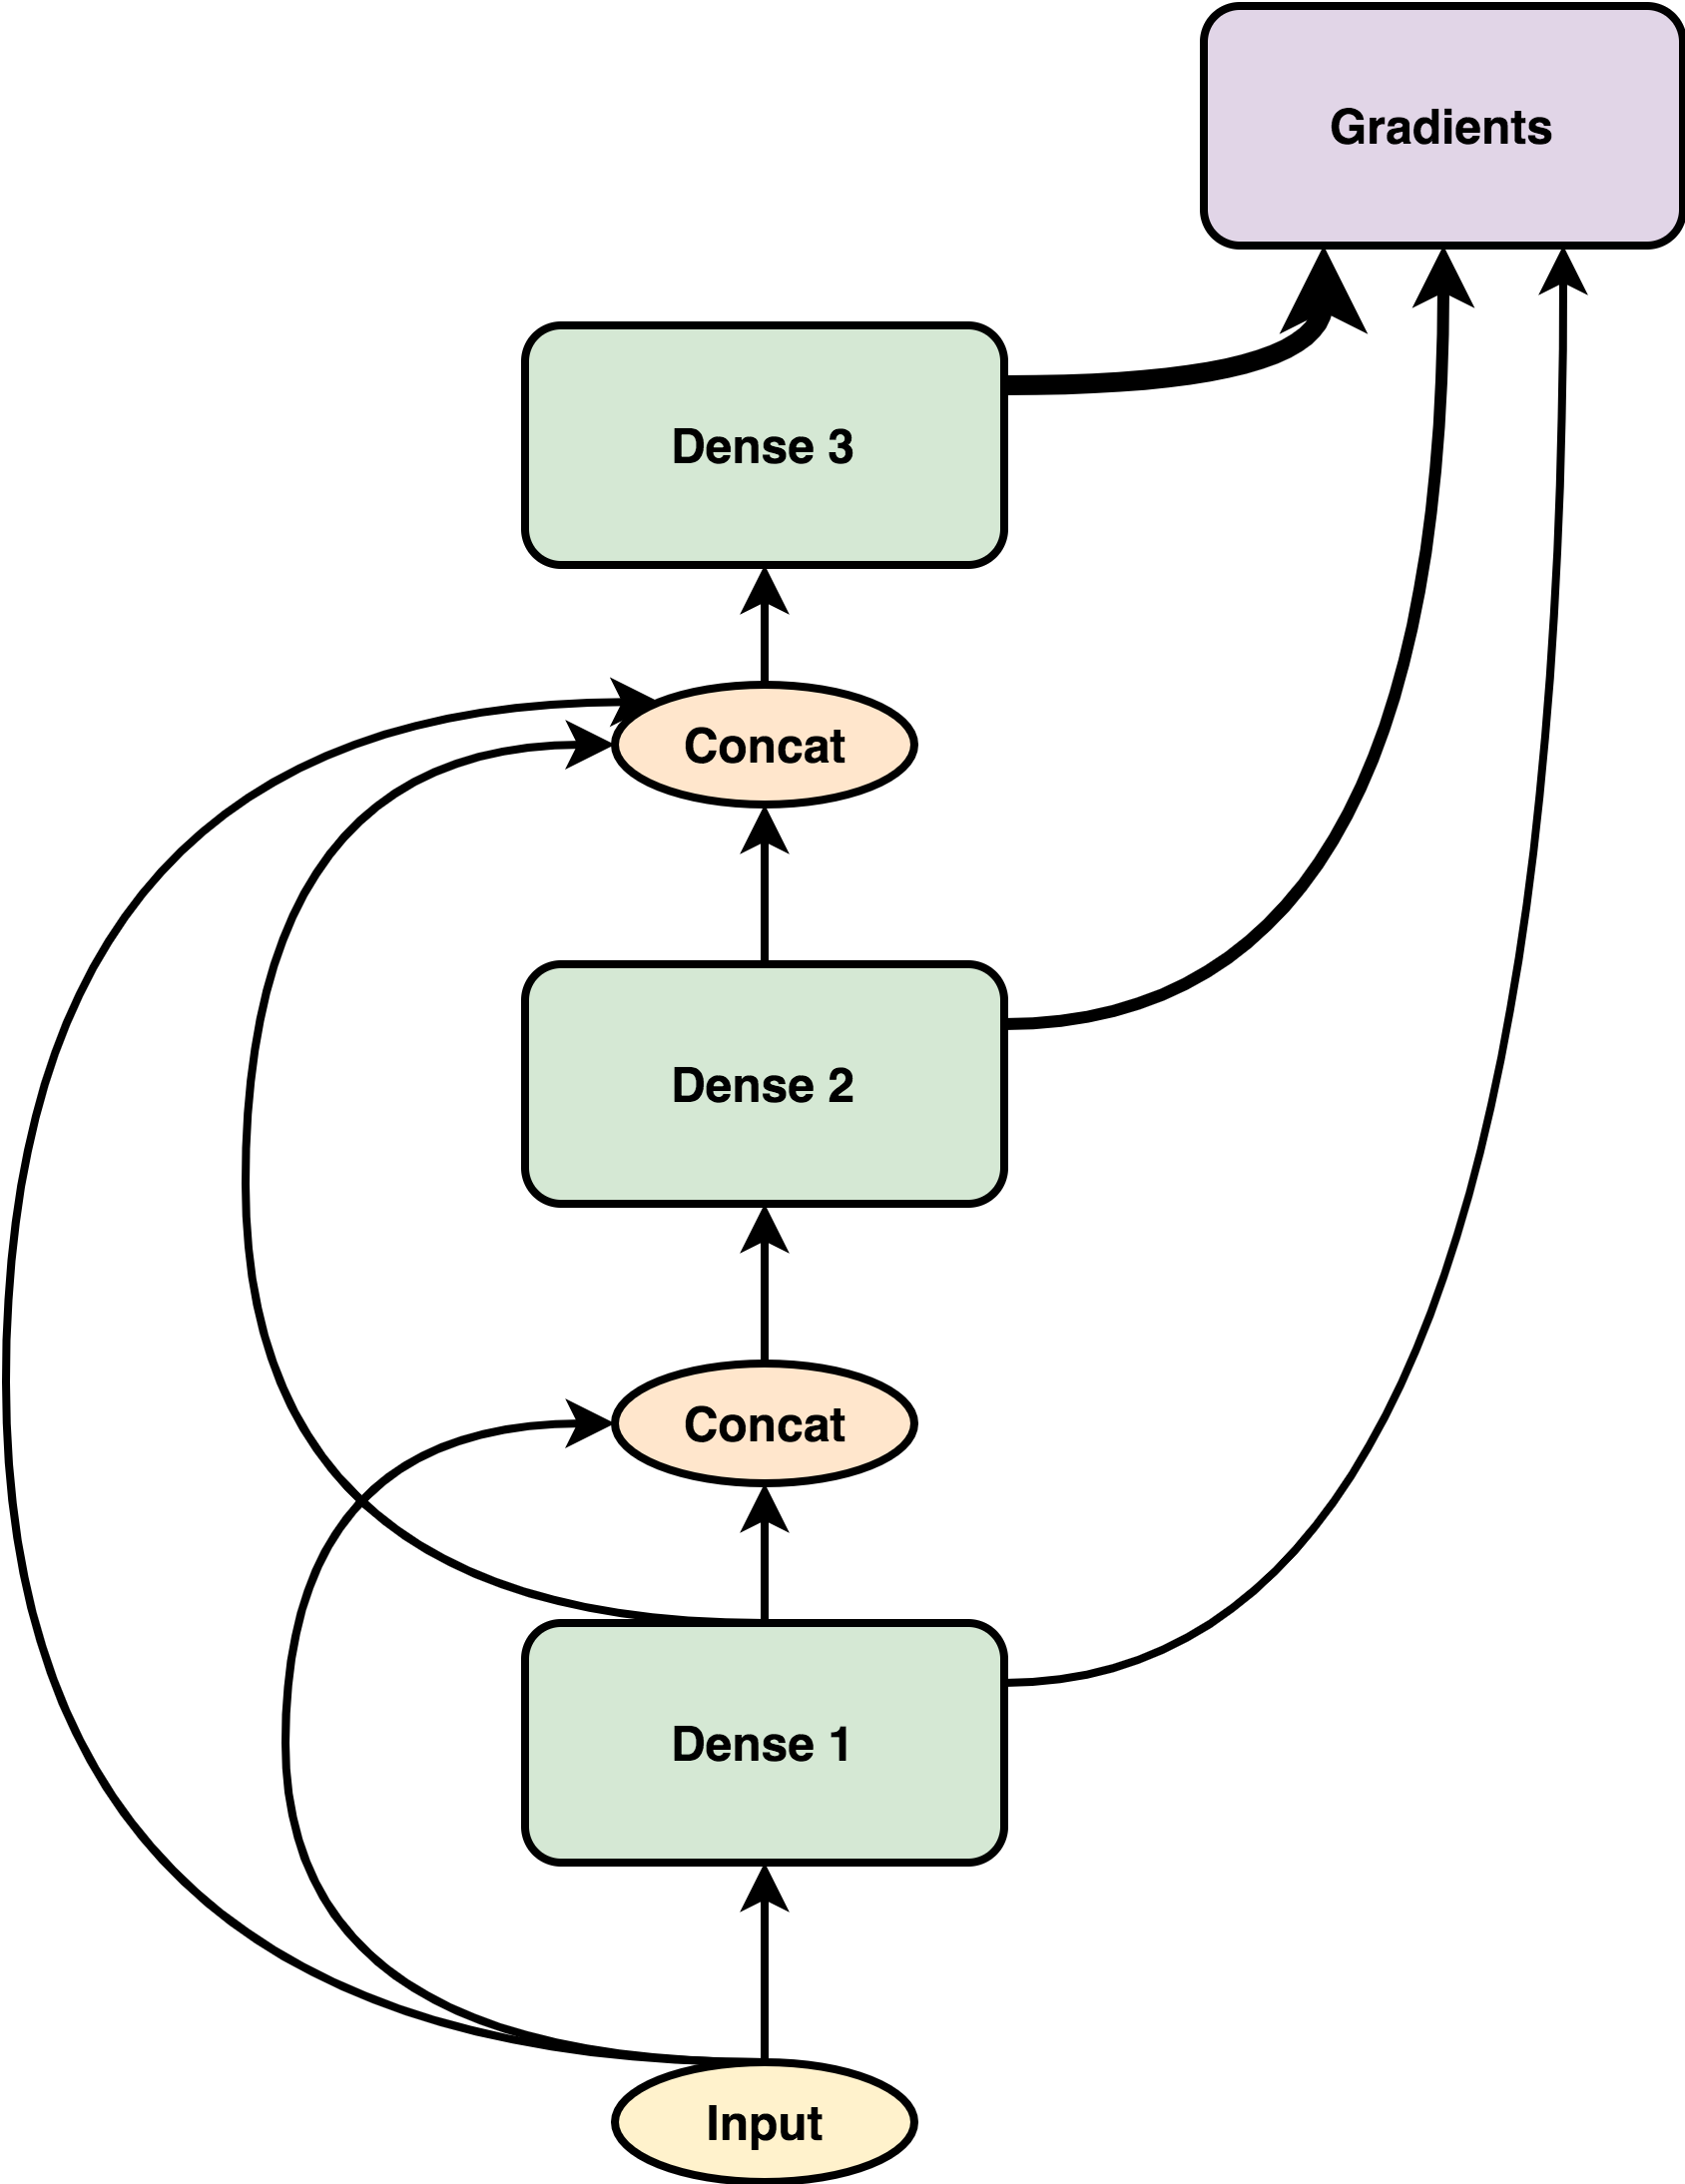
\includegraphics[scale=0.09]{GSC.png}
   \captionof{figure}{Global Short Circuit}
   \label{fig:GSC.png}
\end{minipage}
\begin{minipage}{.45\textwidth}
\begin{equation}
\label{eq:gsc_math_representation}
\begin{aligned}
       Dense_{1} &= \sigma(Input \cdot \hat{W}_{1} + \hat{b}_{1}) &\\
       Dense_{2} &= \sigma([Input \oplus Dense_{1}] \cdot \hat{W}_{2} + \hat{b}_{2}) &\\
       Dense_{3} &= \sigma([Input \oplus Dense_{1} \oplus Dense_{2}] \cdot \hat{W}_{3} + \hat{b}_{3}) 
\end{aligned}
\end{equation}
\end{minipage}

We conduct to experiments show GSC performs better than standard architecture on various datasets. This is due to increased representational capacity of the network. A layer \emph{n} in the network now has access to every other \emph{n-1} previous outputs. This change paves way to create much deeper constructs and complex relationships among the layers. To advocate that the proposed method - GSC creates much deeper constructs than standard architecture, the class confidence of the predictions is measured. Confidence score is unique for each class and the use of \emph{Softmax} function restricts the score between 0 and 1. At the end of each epoch, mean of class confidence score is calculated across a large unseen test set. This measure speaks for the trust in the prediction. Among the variable factors of the measure, the rate of increase and the actual value are vital for the analysis. MNIST \cite{LeCun1998GradientbasedLA}, Fashion-MNIST \cite{Xiao2017FashionMNISTAN}, CIFAR-10 datasets \cite{Krizhevsky2009LearningML} are chosen to account for the variability in the pattern complexity. The training samples are restricted to 10\% of the whole, while still maintaining a large test sample to test the described hypothesis. Figure \ref{fig:cscore_100p_model.png} shows the performance when the architectures across standard and GSC are the same, which leads to a 30\% increase in the trainable parameters due to merge operation. To rule out the difference in the trainable parameters as a reason for achieving high confidence scores, we create 10p architectures. Here, the architecture across the models vary but the number of trainable parameters are kept constant across all architectures(FeedForward, GSC, DSC). The performance of 10p architectures are shown in Figure \ref{fig:cscore_10p_model.png}.  

\noindent\begin{minipage}{.5\textwidth}
   \centering
   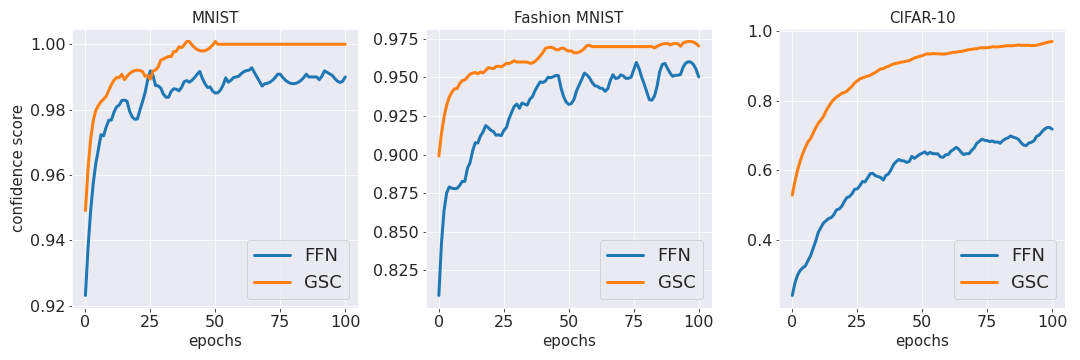
\includegraphics[scale=0.2]{paper/cscore_100p_param.png}
   \captionof{figure}{10p Data, 100p Model}
   \label{fig:cscore_100p_model.png}
   \centering
   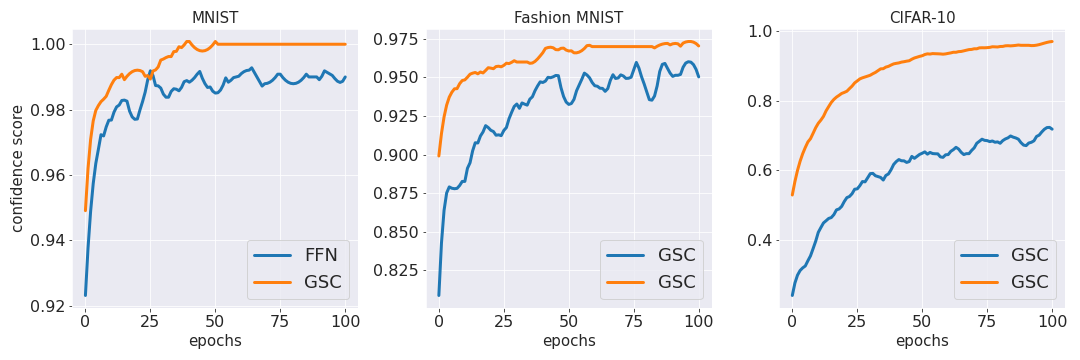
\includegraphics[scale=0.2]{paper/cscore_10p_param.png}
   \captionof{figure}{10p Data, 10p Model}
   \label{fig:cscore_10p_model.png}
\end{minipage}
\begin{minipage}{.4\textwidth}
In figure \ref{fig:cscore_100p_model.png} the difference in the confidence score between that of the standard architecture and GSC is negligable. This is due to the lack of complex patterns across classes in MNIST dataset. Hence, there's a slight difference in the score on Fashion MNIST and a major jump on CIFAR-10. CIFAR-10 comprises of 10 classes of real-world complex object patterns and GSC architecture enables the model to create much deeper constructs compared to the standard architecture. We notice a similar behaviour in the confidence measure across 10p architectures where the number of trainable parameters across the networks is kept constant.
\end{minipage}


However, GSC suffers from an exponential increase in connections resulting in delayed training time. A rise in the number of stacked layers is noticed with the increase in the complexity of the network in terms of depth, which is not scalable. Compared to the standard architecture, GSC has a considerable increase in the number of training parameters. This is due to the effect of merge operation of previous $n-1$ layers for every $n$th layer.

\begin{equation}
\label{eq:gsc_params}
Params= \sum_{n=1}^{m}\left[
\underbrace{(\sum_{i=0}^{n}L_{i}\rule[-12pt]{0pt}{5pt}}_{\mbox{merged inputs}}
*\underbrace{L_{n})\rule[-12pt]{0pt}{5pt}}_{\mbox{weights}}
+\underbrace{L_{n}\rule[-12pt]{0pt}{5pt}}_{\mbox{bias}}\right]
\end{equation}

For the aforementioned 3 layer network, an exponential increase of 30\% i.e, 122,750 parameters has to be trained.

\subsection{Differentiable Short Circuit}
Finally, we proposes Differentiable Short Circuit (DSC) to counter the effect of exponential increase in training parameters due to merge operation. It is done so by expressing a connection between layers as a weighted sigmoid gate. We introduce a connection weight $\hat{C}$, a trainable parameter whose gradients are updated by $\frac{\partial loss}{\partial \hat{C}}$. A change in the value of the connection weight affects the loss. Based on this, we use gradient descent algorithm to obtain optimum values of connection weight. The direction and magnitude of the weight affects the performance of the network by introducing unwanted changes in the architecture. In order to check these effects, a transformation function that is capable of restricting the direction and magnitude of the weight in a specified range is used. Neural arithmetic logic unit \cite{Trask2018NeuralAL} propose a layer whose transformation matrix $\hat{W}$ consists just of -1's, 0's and 1's. In order to prevent the layer from changing the scale of the representation of the numbers when mapping the input to the output, a squashing non-linearity ($\sigma$) is applied on just the weights, $\hat{W}$.  Hence, a sigmoid function, defined in equation \ref{eq:sigmoid_activation}, is applied on $\hat{C}$. Along with forcing the range of output to be in a specific interval, it also helps in preserving the direction of the input. Figure \ref{fig:DSC.png} shows the use of connection weights applied for the results of concat operation, essentially keeping the connection in check before it is fed to the next layer. The difference in representation of connections between various blocks and the gradient operations shows the number of gradient computations required for the layer or the operation. Equations \ref{eq:dsc_math_representation} provides mathematical representation of the network.

\noindent\begin{minipage}{.45\textwidth}
   \centering
   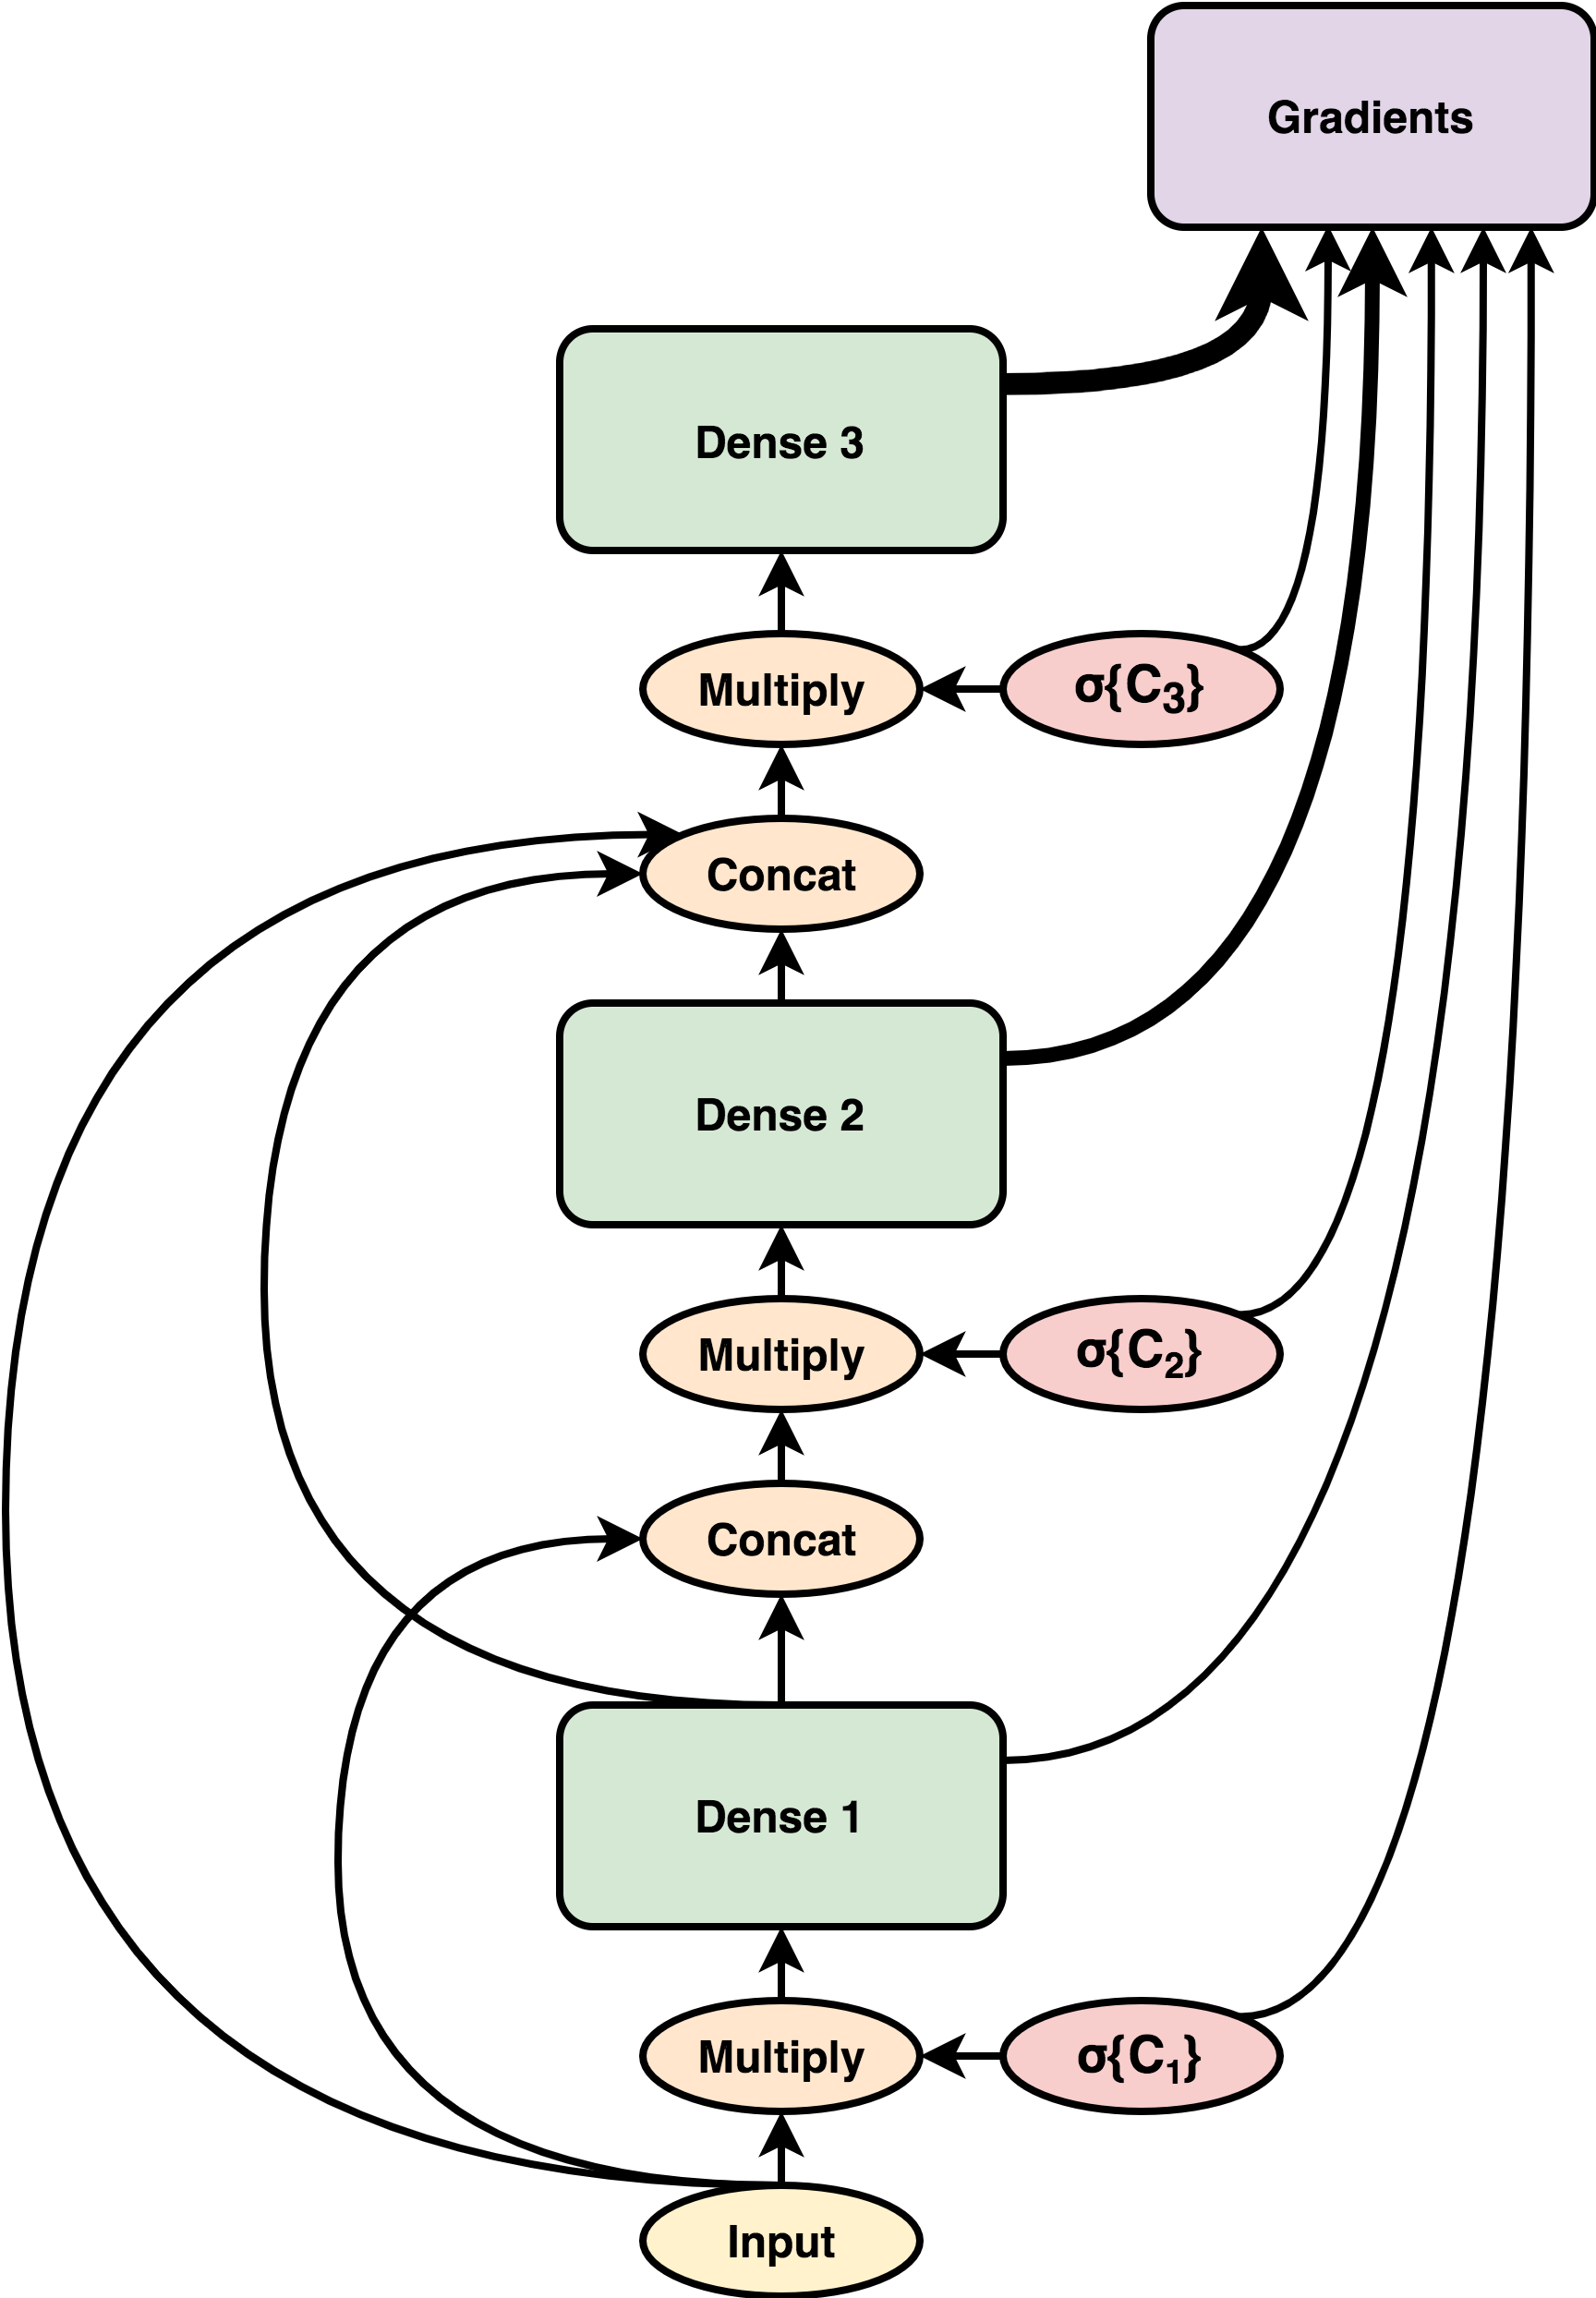
\includegraphics[scale=0.09]{DSC.png}
   \captionof{figure}{Differentiable Short Circuit}
   \label{fig:DSC.png}
\end{minipage}
\begin{minipage}{.45\textwidth}
\begin{equation}
\label{eq:dsc_math_representation}
\begin{aligned}
   Dense_{1} &= \sigma((\sigma(\hat{C}_{1}) \cdot Input) \cdot \hat{W}_{1} + \hat{b}_{1}) &\\
   Dense_{2} &= \sigma((\sigma(\hat{C}_{2}) \cdot [Input \oplus Dense_{1}]) \cdot \hat{W}_{2} + \hat{b}_{2}) &\\
   Dense_{3} &= \sigma((\sigma(\hat{C}_{3}) \cdot [Input \oplus Dense_{1} \oplus Dense_{2}]) \cdot \hat{W}_{3} + \hat{b}_{3}) 
\end{aligned}
\end{equation}
\end{minipage}

For DSC, we notice a slight increase in parameters compared to GSC's equation \ref{eq:gsc_params} due to the use \emph{gates}. There exists a trainable gate for every connection. The number of parameters for connections is defined by $\sum_{i=0}^{n}L_{i}$. As a result, for the network structure defined in the standard architecture, the number of trainable parameters are 124,418, a rise of 1.3\% over GSC.

\begin{equation}
\label{eq:dsc_params}
Params= \sum_{n=1}^{m}\left[
\underbrace{(\sum_{i=0}^{n}L_{i}\rule[-12pt]{0pt}{5pt}}_{\mbox{merged inputs}}
*\underbrace{L_{n})\rule[-12pt]{0pt}{5pt}}_{\mbox{weights}}
+\underbrace{L_{n}\rule[-12pt]{0pt}{5pt}}_{\mbox{bias}}
+\underbrace{\sum_{i=0}^{n}L_{i}\rule[-12pt]{0pt}{5pt}}_{\mbox{connection weights}}\right]
\end{equation}
The benefit of having trainable gates are of two folds,

1. By keeping track of the variance of $\sigma{(\hat{C})}$ over time has proven to be useful in designing a stopping criterion, elucidated in section \ref{sub:InfoTransfer}

2. Since the output of the gates are probabilistic in nature, we use a threshold function to transform continuous values to a binary mask. The mask is used to prune unwanted skip connections. Section \ref{sec:Pruning} describes the pruning methodology in detail.




\subsubsection{Information Transfer Rate}
\label{sub:InfoTransfer}
We also propose \emph{Information transfer rate} (ITR). It is the percentage of measure of data flow from one layer to the next. The gated connections having sigmoid activation translates to a scaling operation. Each output is scaled based on its significance before the same is fed to the next layer. The scaling transformation is also applied to skip connections as shown in figure \ref{fig:DSC.png}. Equation \ref{eq:itr} describes the rate of information transfer from one layer to the next. 

    \begin{equation}
    \label{eq:itr}
    \begin{aligned}
    itr_{layer} &=\frac{\sum_{c=1}^{N}\hat{W}_{c}}{|\hat{W}_{c}|}, \\
    \\
    \text{where}~N &= \text{Number of nodes,} \\
    \hat{W}_{c} &= \text{Connection weight}\\
    |\hat{W}_{c}| &= \text{Length of connection weight}\\
\end{aligned}
\end{equation}

To calculate the information transfer of the network, based on the number of layers and their respective information transfer rates, we propose Equation \ref{eq:itr_mean}.  It is a conditional mean as there are no recurrent associations and connections are always \emph{unidirectional}




\noindent\begin{minipage}{.45\textwidth}
   \centering
   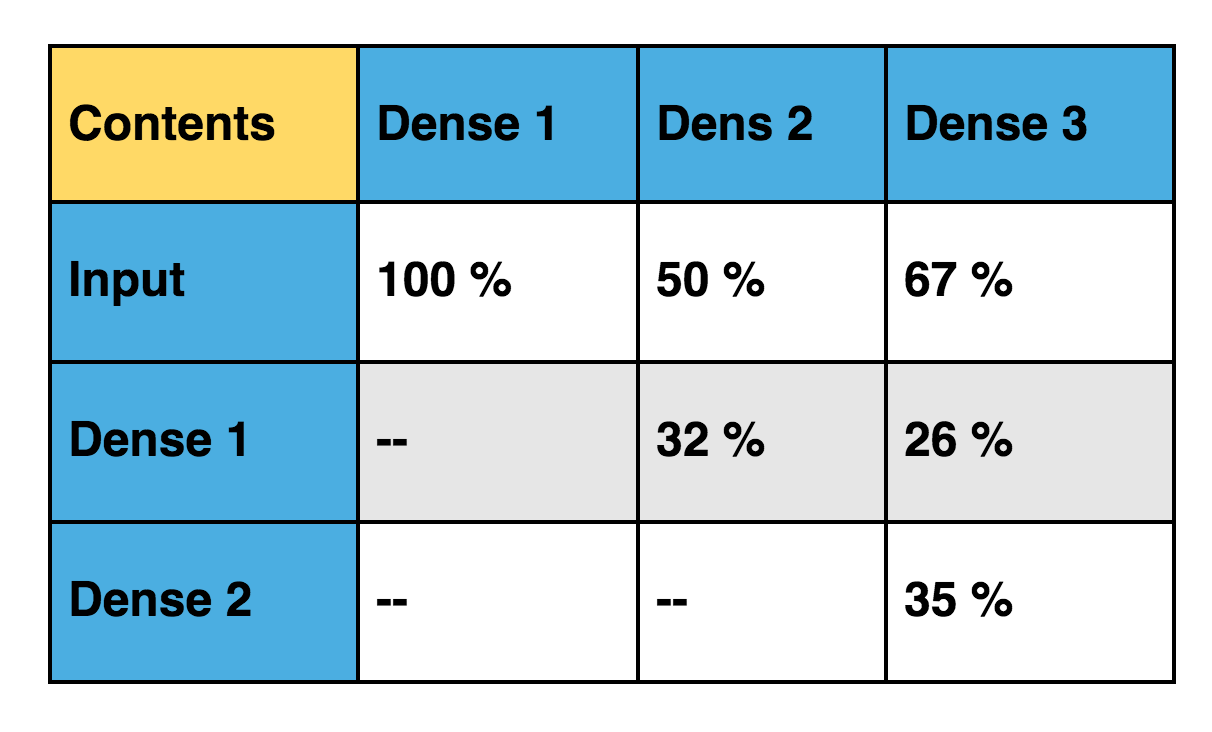
\includegraphics[scale=0.13]{paper/SampleTable.png}
   \captionof{figure}{Sample Infromation Transfer}
   \label{fig:DSC.png}
\end{minipage}
\begin{minipage}{.45\textwidth}
\begin{equation}
\label{eq:itr_mean}
\begin{aligned}
itr_{network} &= \frac{\sum_{i=0}^{n-1}\sum_{j=1}^{n} 
\begin{cases}
  itr_{ij}, & \text{if}\ i<j \\
  0, & \text{otherwise}
\end{cases}}{\frac{n(n+1)}{2}}\\
\text{where}~n &= \text{Number of layers} \\
\end{aligned}
\end{equation}
\end{minipage}


\begin{minipage}{.4\textwidth}
Figure \ref{fig:iv.png} shows that over time, the number of features picked by the network saturates. On a close observation the saturation point of the $itr_{network}$ metric is similar to the saturation point of the accuracy function. MNIST and Fashion MNIST datasets are relatively easy compared to CIFAR-10 and the saturation point of the metric can be used as an early-stopping criterion. In CIFAR-10, the metric changes over time and so does the accuracy and hence it does not meet the early exit criterion.
\end{minipage}
\begin{minipage}{.5\textwidth}
    \centering
    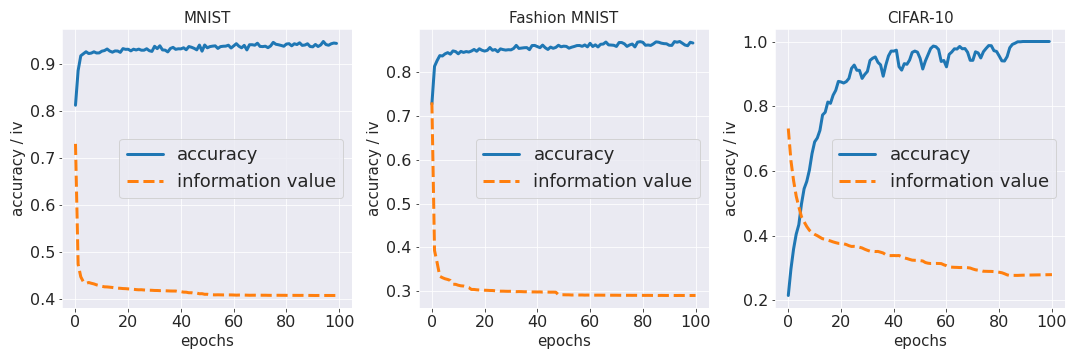
\includegraphics[scale=0.25]{paper/iv.png}
    \captionof{figure}{Information Transfer Rate vs Accuracy}
    \label{fig:iv.png}
\end{minipage}

\subsubsection{Pruning}
\label{sec:Pruning}
To address the issue of exponential increase in trainable parameters due to merge operation in GSC, differentiable short circuit's trainable connection weights are used to selectively prune inessential nodes by removing connections.  If the current input is not important to the task, the value of $\hat{C_{i}}$ will be 0 and the current input information will not be passed on to the next layer. The input to the binary function ranges between 0 and 1. The probability of obtaining 0 or 1 for the binary function can be computed by,
\begin{equation}
\label{eq:ffn_math_representation}
\begin{aligned}
   P(f_{binary(x)}=1) &=x&\\
   P(f_{binary(x)}=0) &=1-P(f_{binary(x)}=1)&\\   
\end{aligned}
\end{equation}
However, the binary connection gate function is not a differentiable function and breaks backpropagation. There are generally two solutions. The first is REINFORCE algorithms \cite{Williams1992SimpleSG} and considering its applications, it is computationally expensive and the reward is difficult to design to approximate the gradients. In recent times, few gradient estimators are proposed and among them, the Straight through gradient estimator \cite{Bengio2013EstimatingOP} is found to be useful due to its reduced computational complexity. The function approximates the step function by the identity when computing gradients during the backward pass:
\begin{equation}
\frac{\partial{f_{binaray}(x)}}{\partial x}=1
\end{equation}
With the implementation of straight through estimator, the model parameters can be trained to optimize the use of connection weights $\hat{C}$ with standard backpropagation without defining any additional supervision or reward signal. This assures that the computation complexity does not increase.

\noindent\begin{minipage}{.5\textwidth}
   \centering
   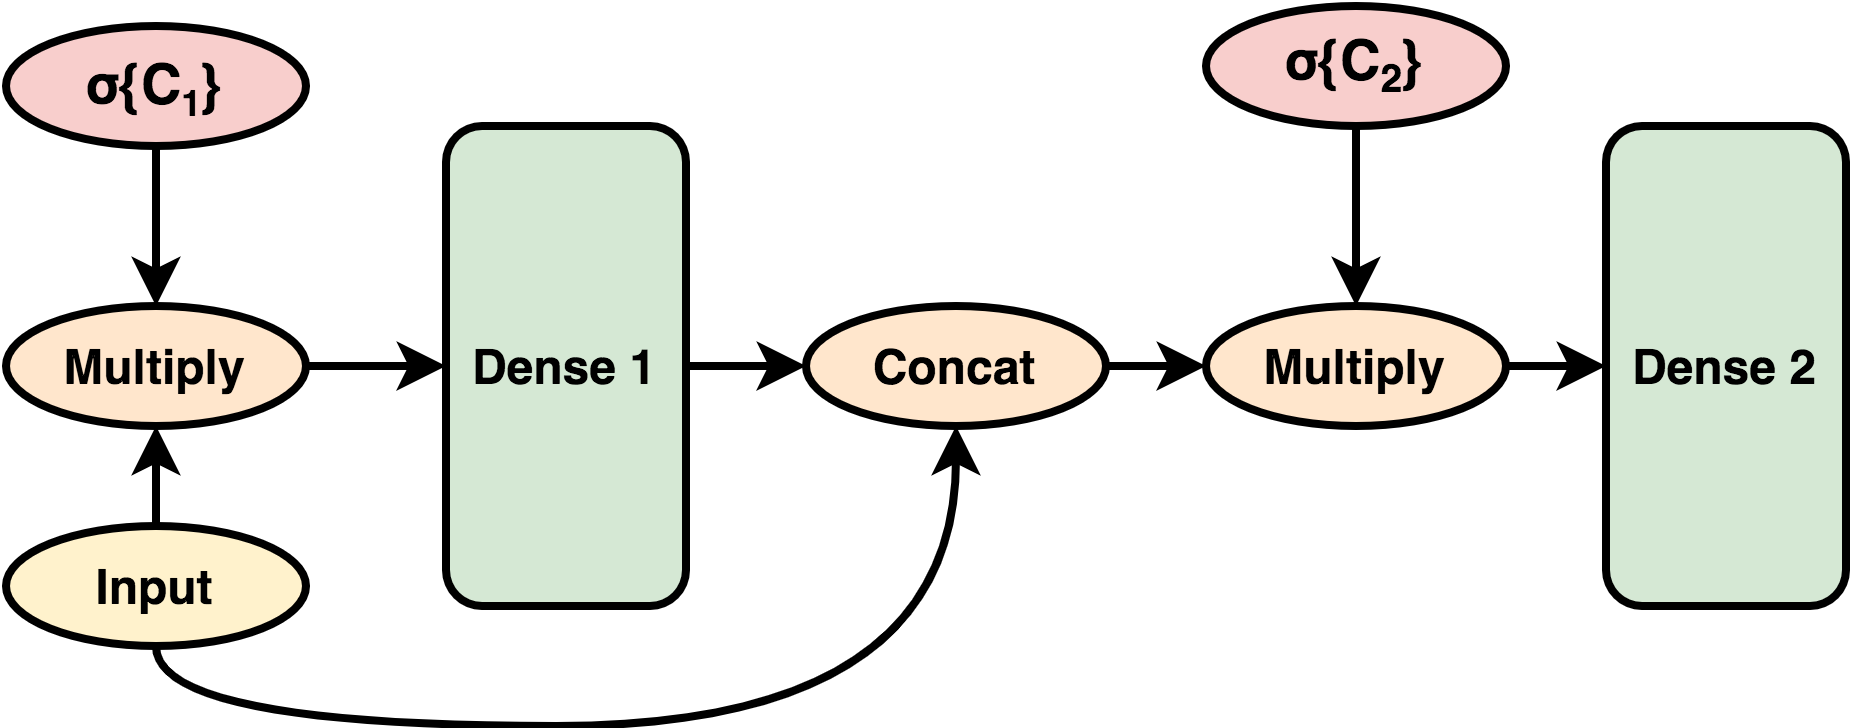
\includegraphics[scale=0.1]{paper/Pruning1.png}
   \captionof{figure}{2-Layer DSC architecture}
%   \label{fig:cscore_100p_model.png}
\end{minipage}
\begin{minipage}{.4\textwidth}
\centering
   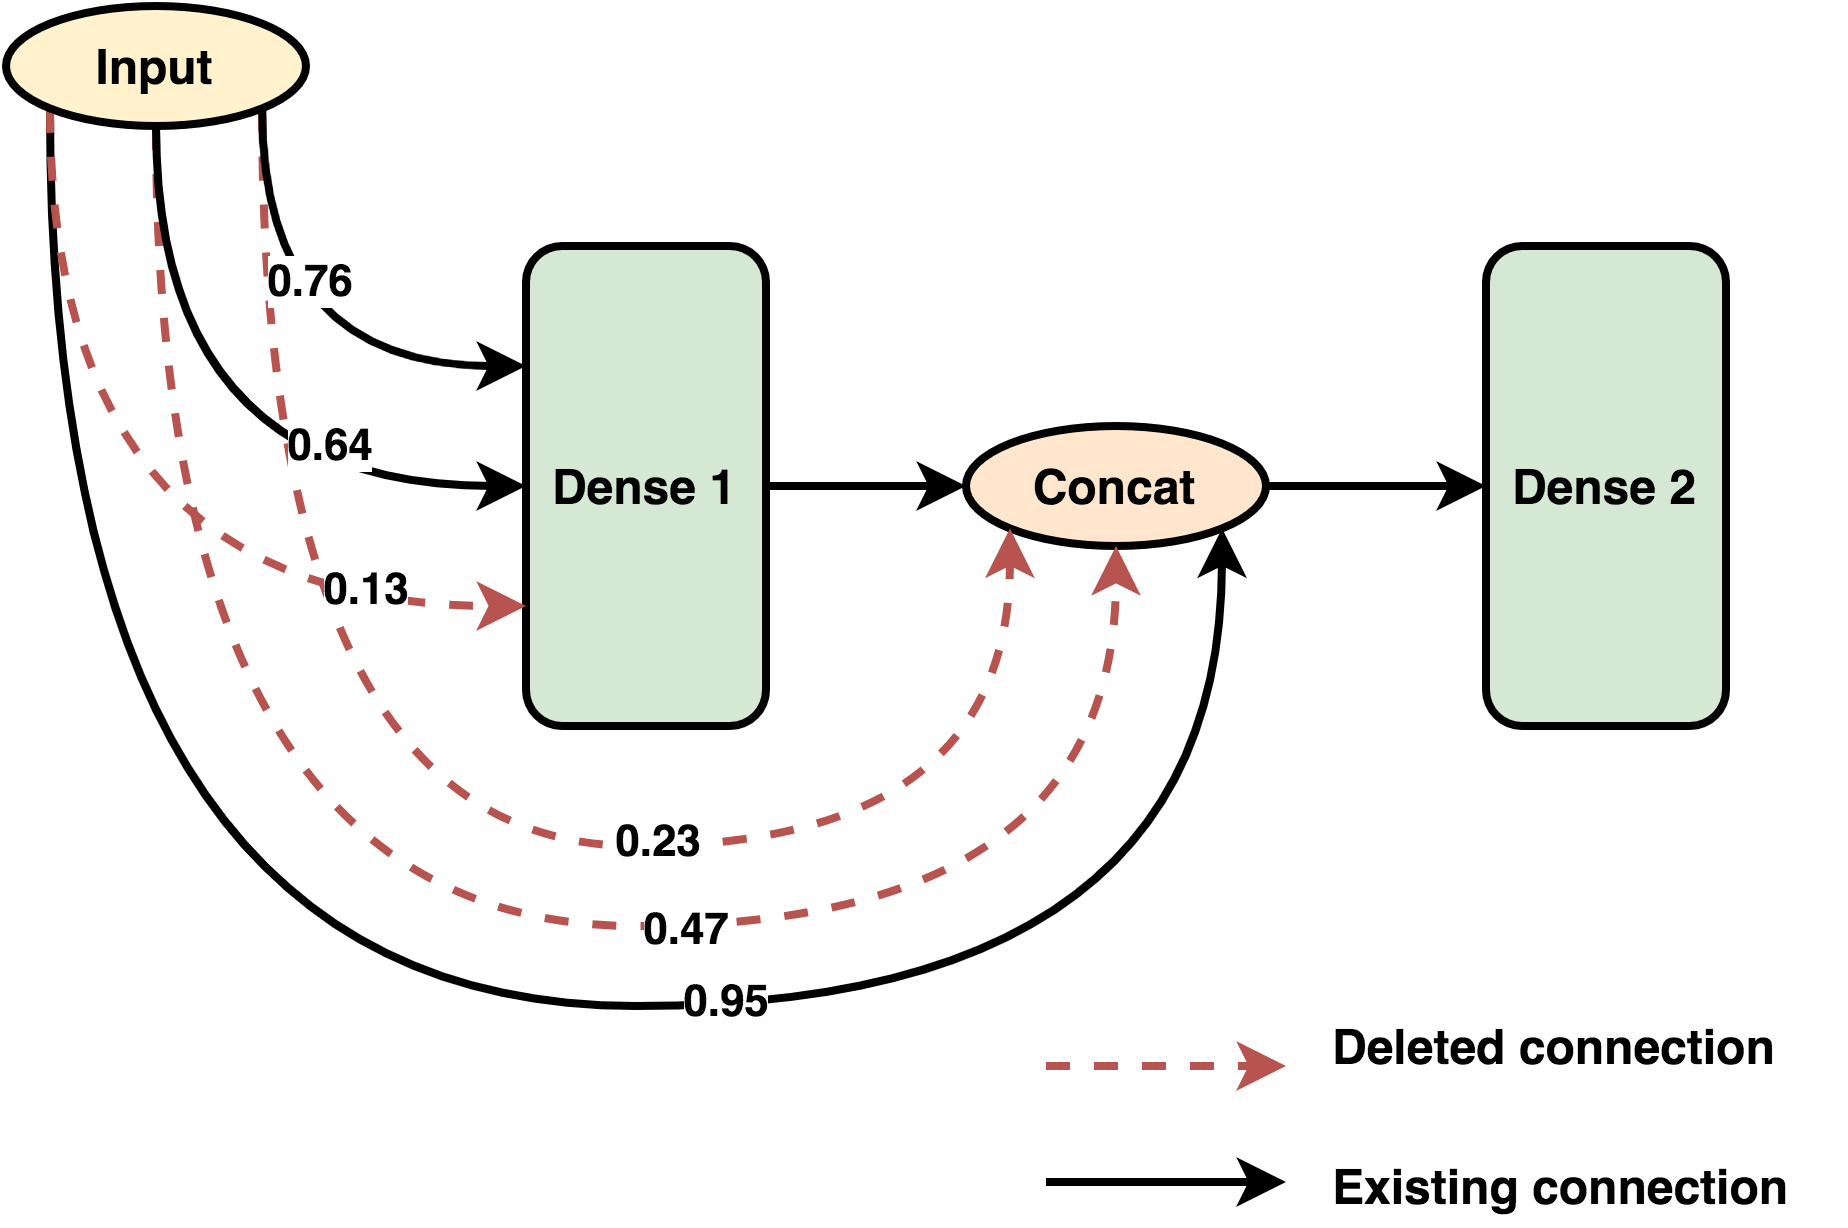
\includegraphics[scale=0.09]{paper/Pruning2.png}
   \captionof{figure}{Pruned connections}
%   \label{fig:c.score_10p_model.png}
\end{minipage}



\noindent\begin{minipage}{.5\textwidth}
  \begin{algorithm}[H]
  
\SetAlgoLined
\KwResult{Prune the network based on binary mask}

\For{layer in network layers;}{
\textit{prune nodes}\textsuperscript{(i)} 	\leftarrow\textit{compute nodes to prune(layer)}

}

i \leftarrow \textit{Number of layers}


 \While{i $<$ 0}{
  \textit{layer} \gets\ \textit{prune}\textit{(layer}\textsuperscript{(i)}, \textit{prune nodes}\textsuperscript{(i)}\textit{)}\

}
 
 \Procedure {prune}{$layer, nodes$}
    \State $layer.weight\gets\ layer.weight[nodes]}$ 
    \State $layer.bias\gets\ {layer.bias[nodes]} $ 
    \State $layer.connections \gets\ layer.connections[nodes]$ 
    \State \textbf{return} $layer$ 
\EndProcedure
 
 
 \caption{Dependency based pruning}
\end{algorithm}

\end{minipage}
\begin{minipage}{.4\textwidth}
In the first for loop we iterate the network layer wise and collect nodes falling under prune criteria and store it in $prune$ $nodes$. We then reverse iterate the network to change layer weights, biases and connection weights based on $prune$ $nodes$. 
\par% 
\bigskip
The $prune$ function takes a layer and the corresponding prune indices and calculates new layer dimensions. It also clones the layer weights, layer bias, connection weights and extracts appropriate indices to match the layer dimensions of the new layer. Finally these new set of parameters are assigned to layer created in the previous step.
\end{minipage}


\section{Experiments}
\label{sec:experiments}

For the experiments, we prefer to use MNIST, Fashion-MNIST and CIFAR-10 datasets. These datasets are chosen based on the complexity of the class patterns. We run hyperparmeter tuning across CV-5 for each of our experiments. This ensures that each network is tuned respectively to get the best performance. We define two sets of data and network architectures,
\begin{itemize}
\item 100p Data - Model is trained on the all of the available training data and is tested against the standard set containing 10,000 samples. This is a standard set to determine the maximum performance of the networks.
\item 10p Data - Model is trained on 10\% of the available training data and is tested against a large set i.e, 10,000 samples. We use this experiment to test our hypothesis - GSC and DSC enables models to develop deep constructs compared to the standard architecture.
\item 100p Params - This set defines a standard architecture for the model design, where the number layers and the number of nodes in the layer are kept constant across architectures. However, we see a 30\% rise in trainable parameters for GSC and DSC architectures compared to the standard architecture. This is due to the merger operation on skip connections.
\item 10p Params - Here, 10\% of the original DSC's architecture is used. Based on the resulting trainable parameters, the other networks are desinged to match this. Though the architectures are different, the number of trainable parameters are kept constant across the networks in this set. It is designed as a counter to the argument - The difference in the performance of the networks is solely dependent on the number of trainable parameters.
\end{itemize}


\begin{tabular}{cc}
    \begin{minipage}{.5\linewidth}
\centering
\begin{tabular}{@{}llll@{}}
\toprule
\textbf{Dataset} & \textbf{Train} & \textbf{Valid} & \textbf{Test} \\ \midrule
MNIST            & 50000          & 10000          & 10000         \\
Fashion MNIST    & 50000          & 10000          & 10000         \\
CIFAR            & 40000          & 10000          & 10000         \\ \bottomrule
\end{tabular}
   \captionof{table}{100p Data samples}
\label{tab:my-table}
    \end{minipage} &
    \begin{minipage}{.5\linewidth}
    \centering
    \begin{tabular}{@{}llll@{}}
\toprule
\textbf{Dataset} & \textbf{Train} & \textbf{Valid} & \textbf{Test} \\ \midrule
MNIST            & 5000          & 1000          & 10000         \\
Fashion MNIST    & 5000          & 1000          & 10000         \\
CIFAR            & 4000          & 1000          & 10000         \\ \bottomrule
\end{tabular}
\captionof{table}{10p Data samples}
\label{tab:my-table}
    \end{minipage} 
\end{tabular}



\begin{tabular}{cc}
    \begin{minipage}{.5\linewidth}
\centering
\begin{tabular}{@{}llll@{}}
\toprule
\textbf{Model} & \textbf{MNIST} & \textbf{Fashion MNIST} & \textbf{CIFAR-10} \\ \midrule
FFN            & 83550          & 83550                  & 162810            \\
GSC            & 122750         & 122750                 & 224250            \\
DSC            & 124418         & 124418                 & 226448            \\ \bottomrule
\end{tabular}
   \captionof{table}{100p Model Parameters}
\label{tab:my-table}
    \end{minipage} &
    \begin{minipage}{.5\linewidth}
    \centering
    \begin{tabular}{@{}llll@{}}
\toprule
\textbf{Model} & \textbf{MNIST} & \textbf{Fashion MNIST} & \textbf{CIFAR-10} \\ \midrule
FFN            & 32425          & 32425                  & 31215             \\
GSC            & 15800          & 15800                  & 25775             \\
DSC            & 17378          & 17378                  & 27838             \\ \bottomrule
\end{tabular}
\captionof{table}{10p Model Parameters}
\label{tab:my-table}
    \end{minipage} 
\end{tabular}


\subsection{100p Data - Large Training Data, Large Test Data}

\begin{figure}[h!]
\centering
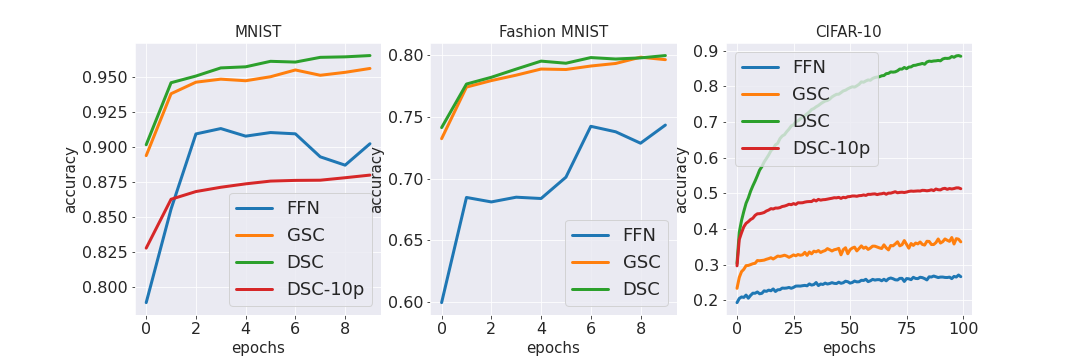
\includegraphics[scale=0.4]{paper/100p_runs.png}
\caption{100p Train comparison}
\label{fig:infotransfer}
\end{figure}

\begin{table}[H]
\centering
\begin{tabular}{llllll}
\hline
\multirow{2}{*}{\textbf{Model}}   & \multirow{2}{*}{\textbf{Parameter}} & \multirow{2}{*}{\textbf{Dataset}} & \multicolumn{2}{c}{\textbf{Train}}                & \multicolumn{1}{c}{\textbf{Test}} \\ \cline{4-6} 
                                  &                                     &                                   & \textbf{Accuracy @ Steps} & \textbf{Loss @ Steps} & \textbf{Accuracy}                 \\ \cline{1-3}
\multirow{3}{*}{Linear FFN}       & \multirow{3}{*}{83550}          & MNIST                    & 0.90 @ 7000          & 0.02 @ 7000          & 0.91                     \\
                                  &                                 & FashionMNIST             & 0.74 @ 7000          & 0.05 @ 7000          & 0.74                     \\
                                  &                                 & CIFAR-10                 & 0.27 @ 7000          & 1.87 @ 7000          & 0.20                     \\
                                  &                                 &                          &                      &                      &                          \\
\multirow{3}{*}{GSC}              & \multirow{3}{*}{122750}         & MNIST                    & 0.93 @ 1400          & 0.0113 @1400         & 0.93                     \\
                                  &                                 & FashionMNIST             & 0.72 @ 700           & 0.0481 @ 700         & 0.79                     \\
                                  &                                 & CIFAR-10                 & 0.28 @ 2100          & 2.53 @ 7000          & 0.29                     \\
                                  &                                 &                          &                      &                      &                          \\
\textbf{DSC}                      & \textbf{124418}                 & \textbf{MNIST}           & \textbf{0.95 @ 1400} & \textbf{0.01 @ 1400} & \textbf{0.96}            \\
\textbf{}                         & \textbf{}                       & \textbf{FashionMNIST}    & \textbf{0.74 @ 700}  & \textbf{0.05 @ 700}  & \textbf{0.79}            \\
\textbf{}                         & \textbf{}                       & \textbf{CIFAR-10}        & \textbf{0.3 @ 700}   & \textbf{2.1 @ 700}   & \textbf{0.40}            \\
                                  &                                 &                          &                      &                      &                          \\
\multirow{3}{*}{\textbf{DSC-10p}} & \multirow{3}{*}{\textbf{17378}} & \textbf{MNIST}           & \textbf{0.89 @ 2800} & \textbf{0.02 @ 2100} & \textbf{0.89}            \\
                                  &                                 & \textbf{FashionMNIST}    & \textbf{0.71 @ 700}  & \textbf{0.07 @ 700}  & \textbf{0.74}            \\
                                  &                                 & \textbf{CIFAR-10}        & \textbf{0.29 @ 700}  & \textbf{2.2 @ 700}   & \textbf{0.38}            \\ \cmidrule(l){3-6} 
\end{tabular}
\caption{100\% Data}
\label{tab:my-table}
\end{table}







\subsection{10p Data - Minimal Training Data, Large Test Data}
\begin{figure}[h!]
\centering
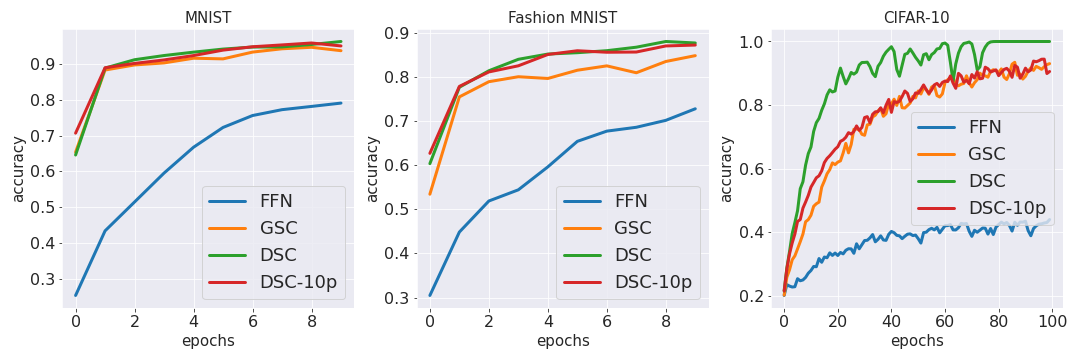
\includegraphics[scale=0.4]{paper/10p_runs.png}
\caption{10p Train comparison}
\label{fig:infotransfer}
\end{figure}


% Please add the following required packages to your document preamble:
% \usepackage{multirow}
\begin{table}[H]
\centering
\begin{tabular}{llllll}
\hline
\multirow{2}{*}{\textbf{Model}}   & \multirow{2}{*}{\textbf{Parameter}} & \multirow{2}{*}{\textbf{Dataset}} & \multicolumn{2}{c}{\textbf{Train}}                & \multicolumn{1}{c}{\textbf{Test}} \\ \cline{4-6} 
                                  &                                     &                                   & \textbf{Accuracy @ Steps} & \textbf{Loss @ Steps} & \textbf{Accuracy}                 \\ \cline{1-3}
\multirow{3}{*}{Linear FFN}       & \multirow{3}{*}{83550}              & MNIST                             & 0.79 @ 7000               & 0.70 @ 7000           & 0.74                              \\
                                  &                                     & FashionMNIST                      & 0.72 @ 7000               & 0.70 @ 7000           & 0.7                               \\
                                  &                                     & CIFAR-10                          & 0.44 @ 7000               & 1.45 @ 7000           & 0.22                              \\
                                  &                                     &                                   &                           &                       &                                   \\
\multirow{3}{*}{GSC}              & \multirow{3}{*}{122750}             & MNIST                             & 0.79 @ 2100               & 0.69 @ 2100           & 0.85                              \\
                                  &                                     & FashionMNIST                      & 0.72 @ 2100               & 0.70 @ 2100           & 0.76                              \\
                                  &                                     & CIFAR-10                          & 0.44 @ 700                & 2.46 @ 700            & 0.28                              \\
                                  &                                     &                                   &                           &                       &                                   \\
\textbf{DSC}                      & \textbf{124418}                     & \textbf{MNIST}                    & \textbf{0.88 @ 1400}      & \textbf{2.13 @ 1400}  & \textbf{0.89}                     \\
\textbf{}                         & \textbf{}                           & \textbf{FashionMNIST}             & \textbf{0.77 @ 1400}      & \textbf{1.91 @ 1400}  & \textbf{0.79}                     \\
\textbf{}                         & \textbf{}                           & \textbf{CIFAR-10}                 & \textbf{0.64 @ 700}       & \textbf{1.05 @ 700}   & \textbf{0.33}                     \\
                                  &                                     &                                   &                           &                       &                                   \\
\multirow{3}{*}{\textbf{DSC-10p}} & \multirow{3}{*}{\textbf{17378}}     & \textbf{MNIST}                    & \textbf{0.75 @ 700}       & \textbf{1.56 @ 700}   & \textbf{0.87}                     \\
                                  &                                     & \textbf{FashionMNIST}             & \textbf{0.77 @ 1400}      & \textbf{1.51 @ 1400}  & \textbf{0.77}                     \\
                                  &                                     & \textbf{CIFAR-10}                 & \textbf{0.43 @ 700}       & \textbf{1.6 @ 700}    & \textbf{0.26}                     \\ \cline{3-6} 
\end{tabular}
\caption{10\% Data}
\label{tab:my-table}
\end{table}





\subsection{Understanding connection weights ($\hat{C}$)}
To comprehend the nature of gated connections, we create thresholded heatmaps of the weights. This is possible since connection weight is a function of $\sigma$ and only skip connections from Input to every other layer is considered. Figure \ref{fig:mnist_vis} and \ref{fig:fashion_mnist_vis} represents connection weights from input to the other three layers defined in section \ref{sec:}. The borders of the input do not contain any valuable information and the network learns to discard these connections over time. The model learns to drop common features among different classes and this reduces class ambiguity and thereby increasing the confidence score of a class. The mean utilization of inputs represents the common used pixels across different class and layers with high importance.

\begin{figure}[H]
\centering
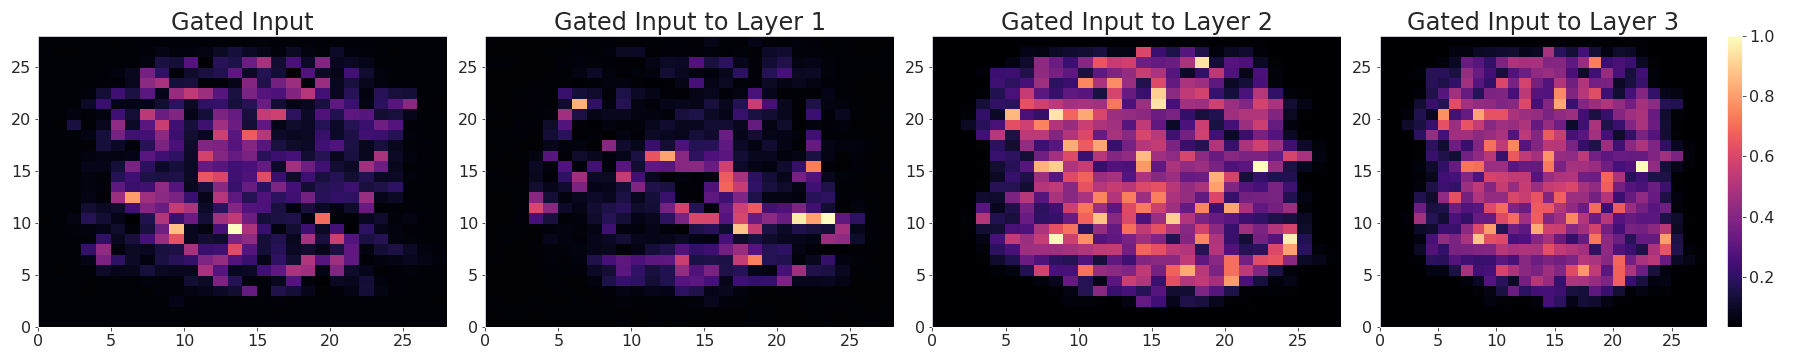
\includegraphics[scale=0.2]{paper/mnist_vis.png}
\captionof{figure}{MNIST Dataset}
\label{fig:mnist_vis}
\end{figure}

\begin{figure}[H]
\centering
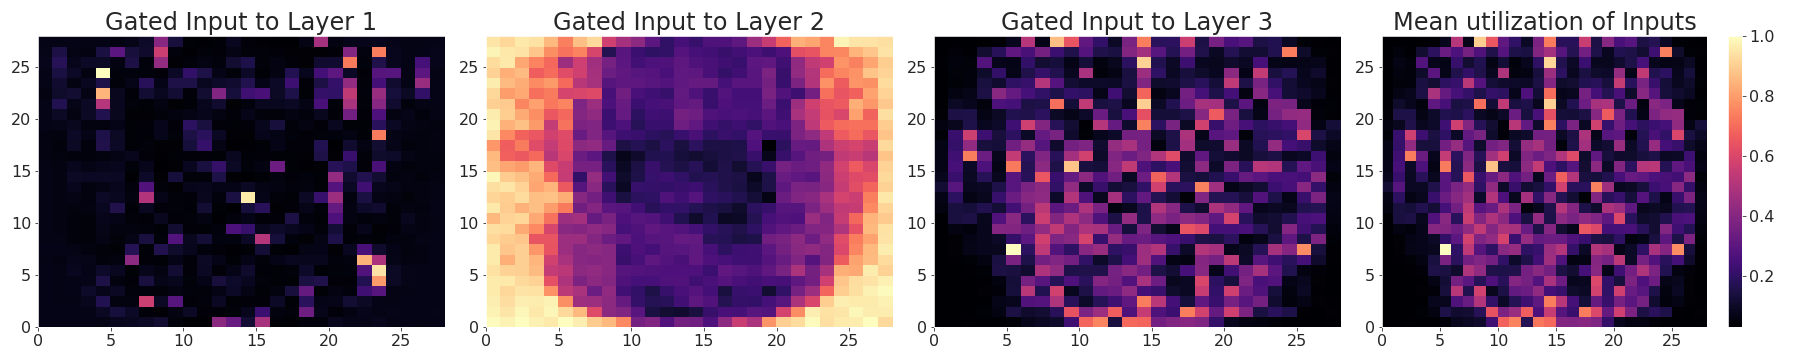
\includegraphics[scale=0.2]{paper/fashionmnist_vis.png}
\captionof{figure}{Fashion MNIST Dataset}
\label{fig:fashion_mnist_vis}
\end{figure}

\section{Conclusion}

Our work establishes the usefulness of global short circuits to improve the performance of the network by enabling the model to develop much deeper constructs compared to the standard architecture. We elucidate issues with global short circuit and propose differentiable short circuit as a solution. Differentiable short circuit builds upon GSC  with the goal of scalability. DSC archiecture with the help of connection weights brings in innovations such as Information Transfer Rate, Pruning, Layer intake visualization among others. The architecture achieves the top accuracy in fewer iterations compared to standard architecture and GSC across all datasets. 

From our experiments we can conclude that DSC reduces model overfit, achieves high training accuracy while still maintaing a relatively high test accuracy. As a counter to the argument - increase in the trainable parameters is solely reponsible to the increase in performance, we design and test a relatively smaller network without deteriorating the performance of the original network. Added benefit is that our proposed method is capable of learning at much faster pace ($learning rate > 0.1$) and with the optimal use of learning rate scheduler, the method achieves local minima in fewer iterations compared to other models. With the help of pruning we  introduce factor of sparsity which is aimed at reducing the number of trainable parameters while still maintianing a fairly high test metrics.



\section{Future Work}

DSC on FeedForward neural networks stands as a testimony proving the proposed new architecture holds water. We see the surge in performance when skip connections along with differentiable connections are introduced. We plan to port t


\bibliographystyle{unsrt}  
\bibliography{references}
\end{document}